% !TEX encoding = UTF-8 Unicode
% !TEX root = thesis-ex.tex
This chapter shall discuss some important experimental jet measurements that motivate the study of the main analysis in this thesis. These include the study of the jet yields, dijet asymmetry, and jet fragmentation. 


\section{Dijet Balance: $\mathrm{x}_{J}$}
\label{sec:xj}
This section will discuss the dijet balance for $R = 0.4$ jets as measured by ATLAS detector for \pbpb\ collisions at \sqrtsnn = 2.76 TeV \cite{Aaboud:2017eww}. The dijet imbalance can be expressed in terms of $x_J$ defined as

\begin{align}
x_J =  \frac{\pt_2}{\pt_1}
\end{align}

where $\pt_2$ and $\pt_1$ are the transverse momenta of the two highest-\pt\ jets in the event respectively. The minimum $\pt_2$ considered is 25 GeV and the pair of jets are separated by $|\Delta\phi| > 7\pi/8$. The dijet yields normalized by the number of jets and determined as $1/N_\mathrm{jets} dN/dx_J$ are presented as a function of $x_J$ for different centrality intervals, as well as different ranges for $\pt_1$. The measured distributions are further unfolded to remove detector resolution effects and allow comparison to theoretical models.

Figure~\ref{fig:xJ} shows the $x_J$ distribution for dijet pairs in \pp\ and \pbpb\ collisions in two different centrality bins and two $\pt_1$ ranges. It can be seen that the dijet yields in \pp\ are peaked at unity and become narrower for larger $\pt_1$ ranges. This reflects the fact that the effects of jet quenching are minimal and the higher-\pt\ jets are better balanced. The dijet yields in peripheral \pbpb\ collisions are similar to the distributions from the \pp\ data, showing that the effects of quenching are smaller. On the other hand, dijet yields in central \pbpb\ collisions are significantly broadened, reflecting the maximal  of jet quenching. This is consistent with the picture of the individual jets in the dijet pair traversing different lengths in the QGP and hence losing different amounts of energy. In fact, the distribution for \pbpb\ data is peaked at $x_J = 0.5$, implying a loss of 50\% of the jet \pt.

\begin{figure}[htbp]
\begin{center}
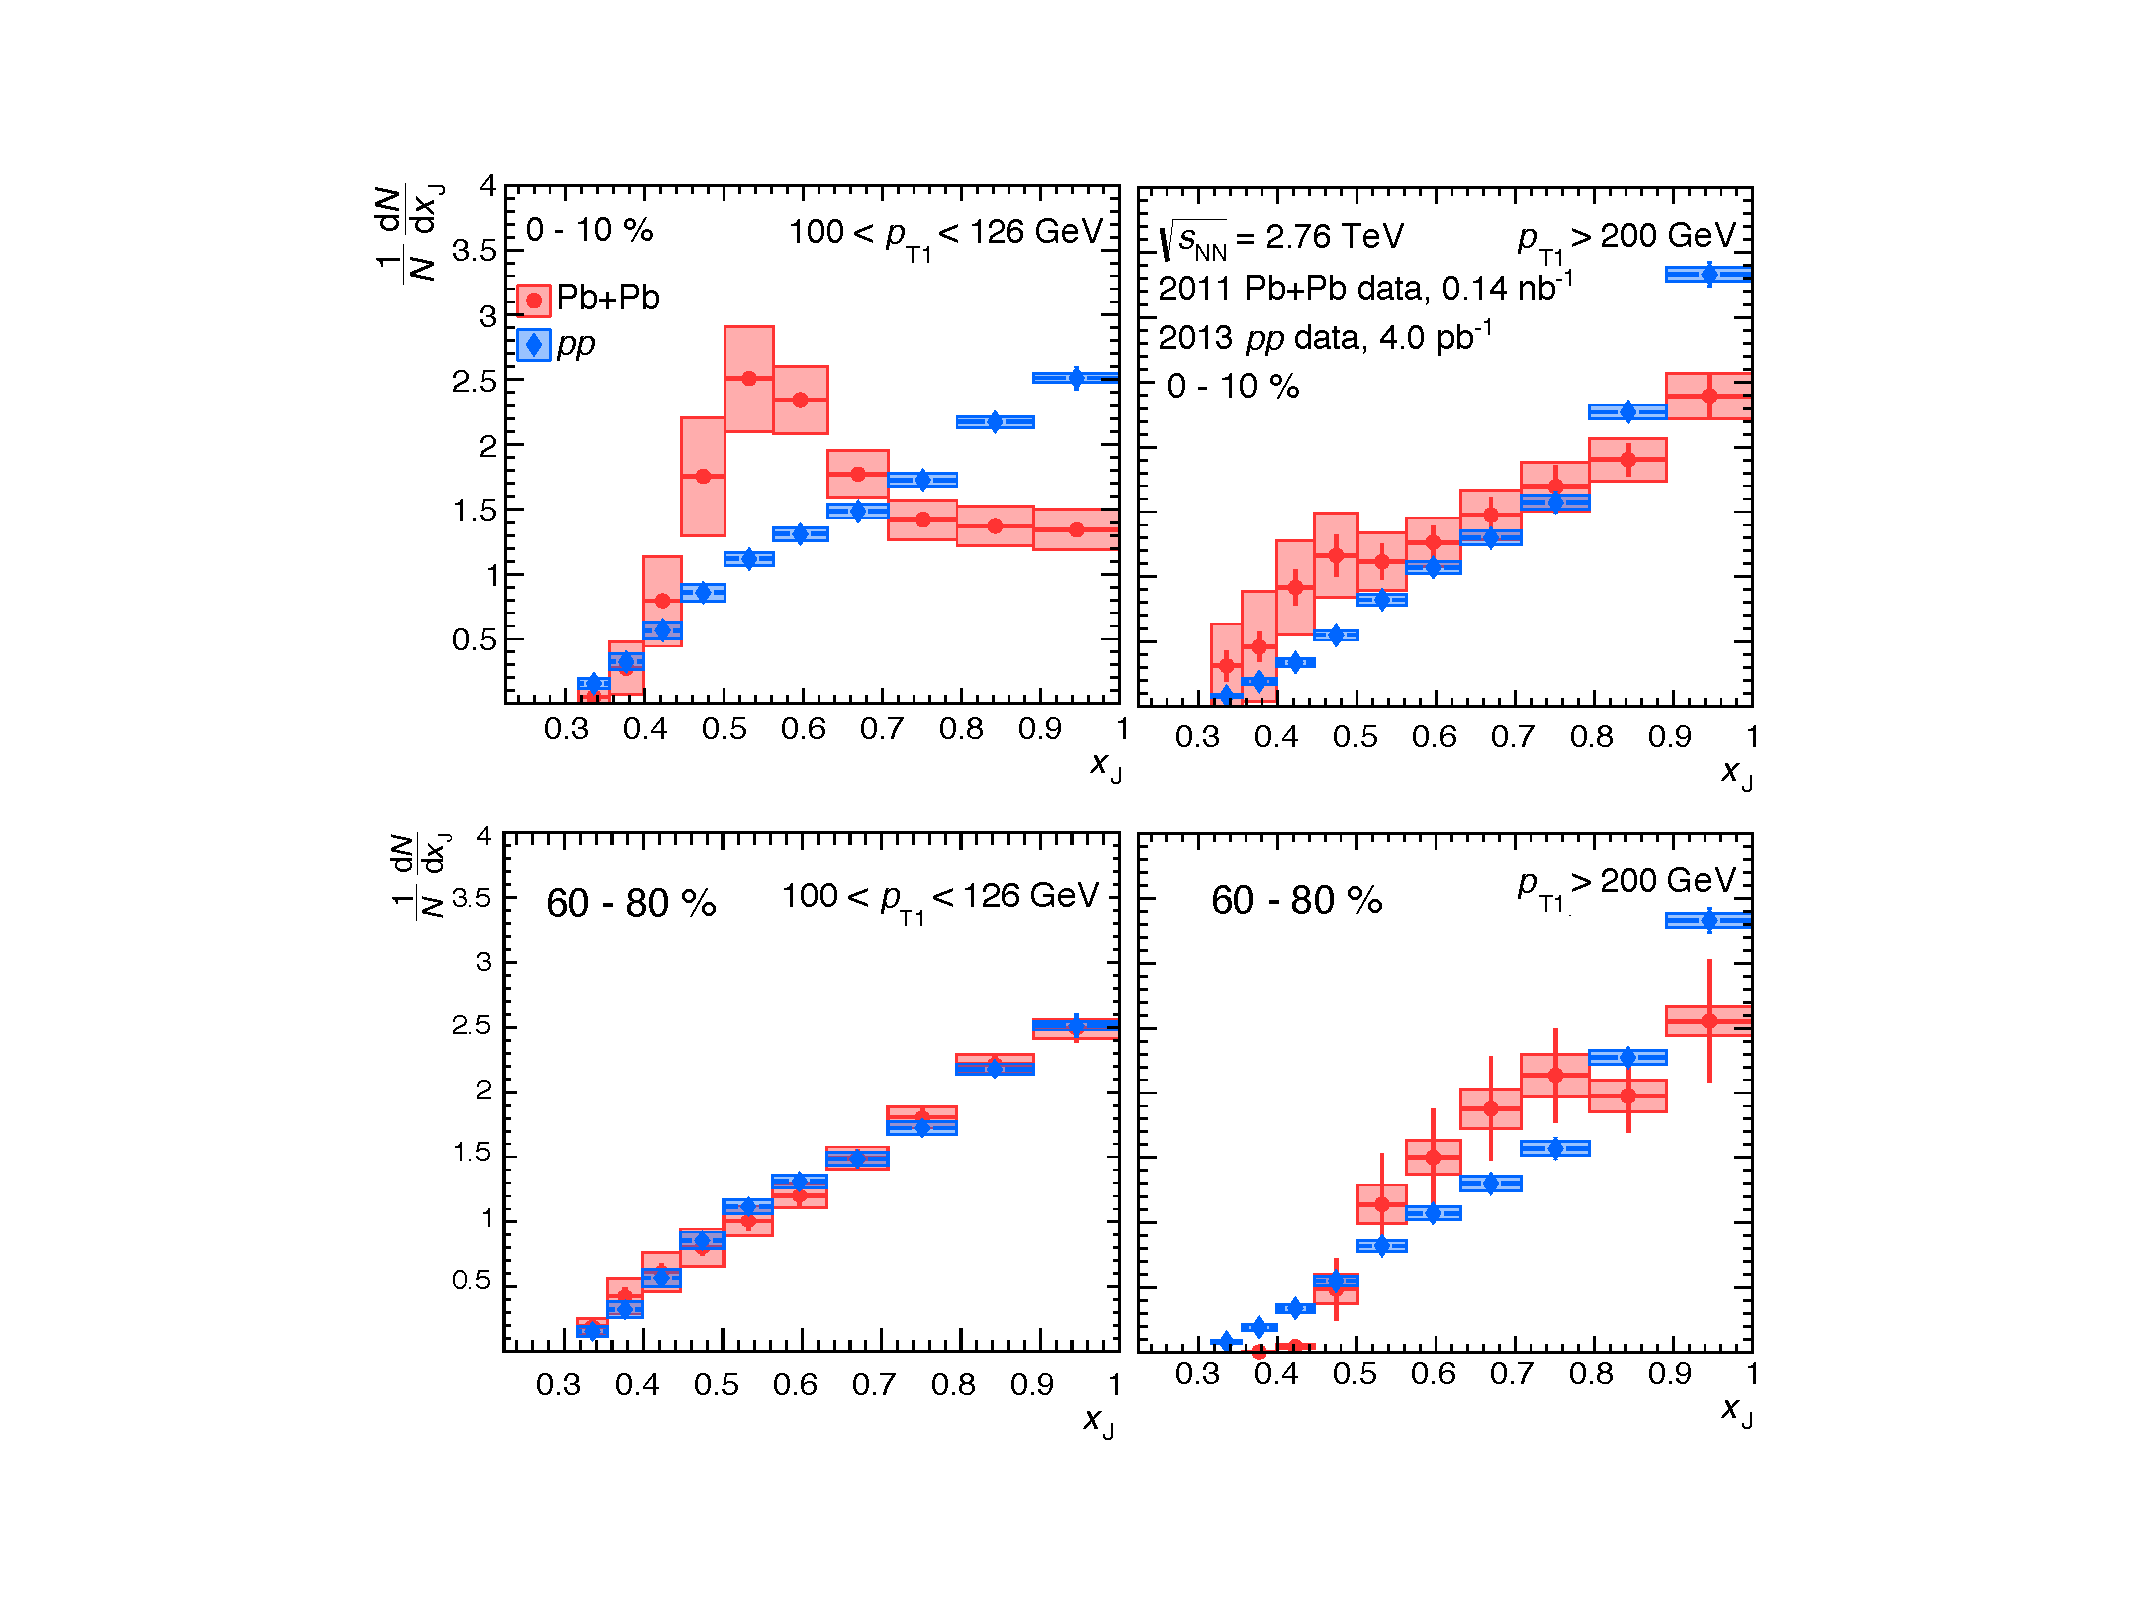
\includegraphics[width=0.55\textwidth]{figures/jetMeasurements/xJ}
\caption{The $1/N_\mathrm{jets} dN/dx_J$ distributions for $R=0.4$ jets as a function of $x_J$ for \pp\ (blue) and \pbpb\ (red) collisions. The different panels are for (top) central and (bottom) peripheral collisions in (left) $100 < \pt_1 < 126$ GeV and (right) $\pt_1 > 200 $ GeV. The \pp\ data is the same in all panels. The statistical uncertainties are indicated by the bars while the boxes indicate the systematic uncertainties. Figures taken from \cite{Aaboud:2017eww}}
\label{fig:xJ}
\end{center}
\end{figure}

Further measurements of $R = 0.3$ jets are shown in Figure~\ref{fig:xJ_R03}. These distributions are significantly flatter than the ones for $R=0.4$ jets, an observation that is consistent with the expectation that the transverse momenta correlation between the dijet pair is weaker for jets with smaller radii due to radiation that is outside the nominal jet cone.

\begin{figure}[htbp]
\begin{center}
\includegraphics[width=0.55\textwidth]{figures/jetMeasurements/xJ_R03}
\caption{The $1/N_\mathrm{jets} dN/dx_J$ distributions for $R=0.3$ jets as a function of $x_J$ in \pp\ and central \pbpb\ collisions. The different panels are for different, $\pt_1$ ranges (top left to bottom right) central and (bottom) peripheral collisions. The \pbpb\ data is in red circles while the \pp\ data is in blue diamonds and is the same in all panels. The statistical uncertainties are indicated by the bars while the boxes indicate the systematic uncertainties. Figures taken from \cite{Aaboud:2017eww}}
\label{fig:xJ_R03}
\end{center}
\end{figure}


\section{Modification of jet yields: $\mathrm{R}_{AA}$}
This section discusses the measurement of the inclusive jet \RAA\ as measured by the ATLAS detector for $R=0.4$ jets in $\sqrtsnn=5.02$ TeV \pbpb\ collisions \cite{2019108}.

While a measurement that compares the jets in a dijet system to each other as discussed in Section~\ref{sec:xj} can provide valuable information about how jets lose energy, it has the following limitation: If both jets lose equal amounts of energy, the dijet yield will still be peaked at unity and no new information will be obtained. Thus, it is useful to compare the jet yields directly between the \pp\ and \pbpb\ systems and construct the jet \RAA\ observable. This is defined as:

\begin{align}
\RAA  = \dfrac{\dfrac{1}{N_{\rm evt}} \left. \dfrac{d^2 N_{\rm jet}}{d\pt dy} \right|_{\rm cent}}{ \langle T_{\rm AA} \rangle \left. \dfrac{d^2\sigma_{\rm jet}}{d\pt dy} \right|_{\rm pp}}
\end{align}

where \TAA is the nuclear thickness function and accounts for the geometric enhancement between \pp\ and \pbpb\ as discussed in Section~\ref{sec:HICollisions} and \cite{doi:10.1146/annurev.nucl.57.090506.123020}. 

This measurement was conducted for jets in the 40--1000 GeV range in different rapidity and centrality intervals. The jet yields in \pp\ and \pbpb\ collisions are shown in Figure~\ref{fig:jet_yields} . The \pbpb\ jet yields are scaled by the thickness function and are shown for 8 centrality intervals. Figure~\ref{fig:raa} shows the measured inclusive jet \RAA\ as a function of jet \pt\ for different centrality bins and jet rapidity $|y| < 2.8$. It can be seen that the most central collisions show a clear suppression with an $\RAA \approx 0.45$ at jet $\pt\ 100$ GeV. The \RAA\ value slowly evolves with jet \pt\ and rises to 0.6 at jet $\pt = 800$ GeV. This modification becomes smaller for more peripheral collisions. The smooth centrality dependence can be more clearly seen in Figure~\ref{fig:raa_centDep}, where \RAA\ is shown as a function of \ANpart\ for jets the 100--126 GeV and 200--251 GeV ranges. The magnitude of the suppression is also seen to depend on jet \pt\ for $\ANpart \geq 50$. 


\begin{figure}[htbp]
\begin{center}
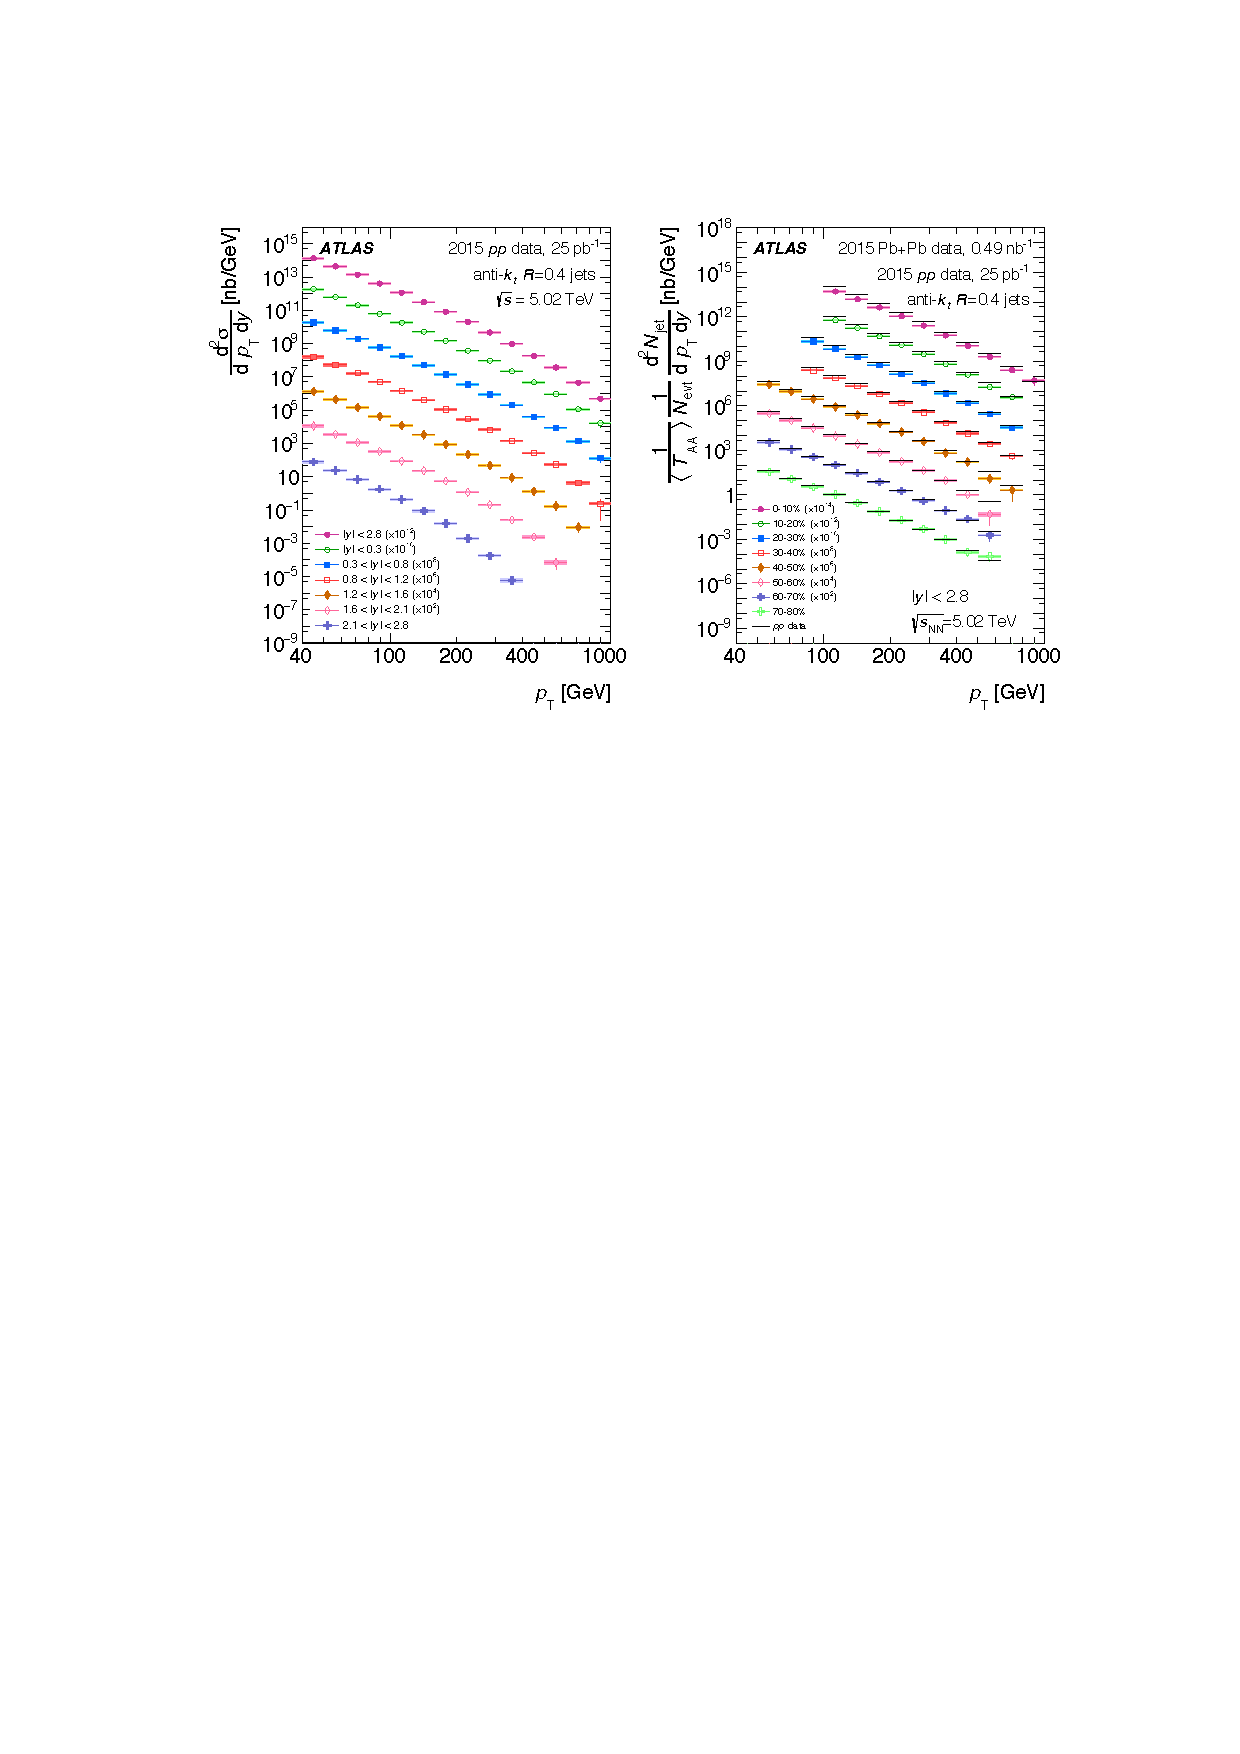
\includegraphics[width=0.85\textwidth]{figures/jetMeasurements/jetYields}
\caption{(Left) The inclusive jet cross section in \pp\ collisions as a function of jet \pt\ in different $|y|$ intervals scaled by successive powers of $10^2$ for visibility. (Right) Per event inclusive jet yield in \pbpb\ collisions normalized by $\langle \TAA \rangle$ as a function of jet \pt\ in different centrality intervals scaled by successive powers of $10^2$ for visibility. The solid lines represent the cross section from \pp\ data at the same rapidity interval scaled by the same $10^2$ factor.  Figure taken from \cite{2019108}}
\label{fig:jet_yields}
\end{center}
\end{figure}


\begin{figure}[htbp]
\begin{center}
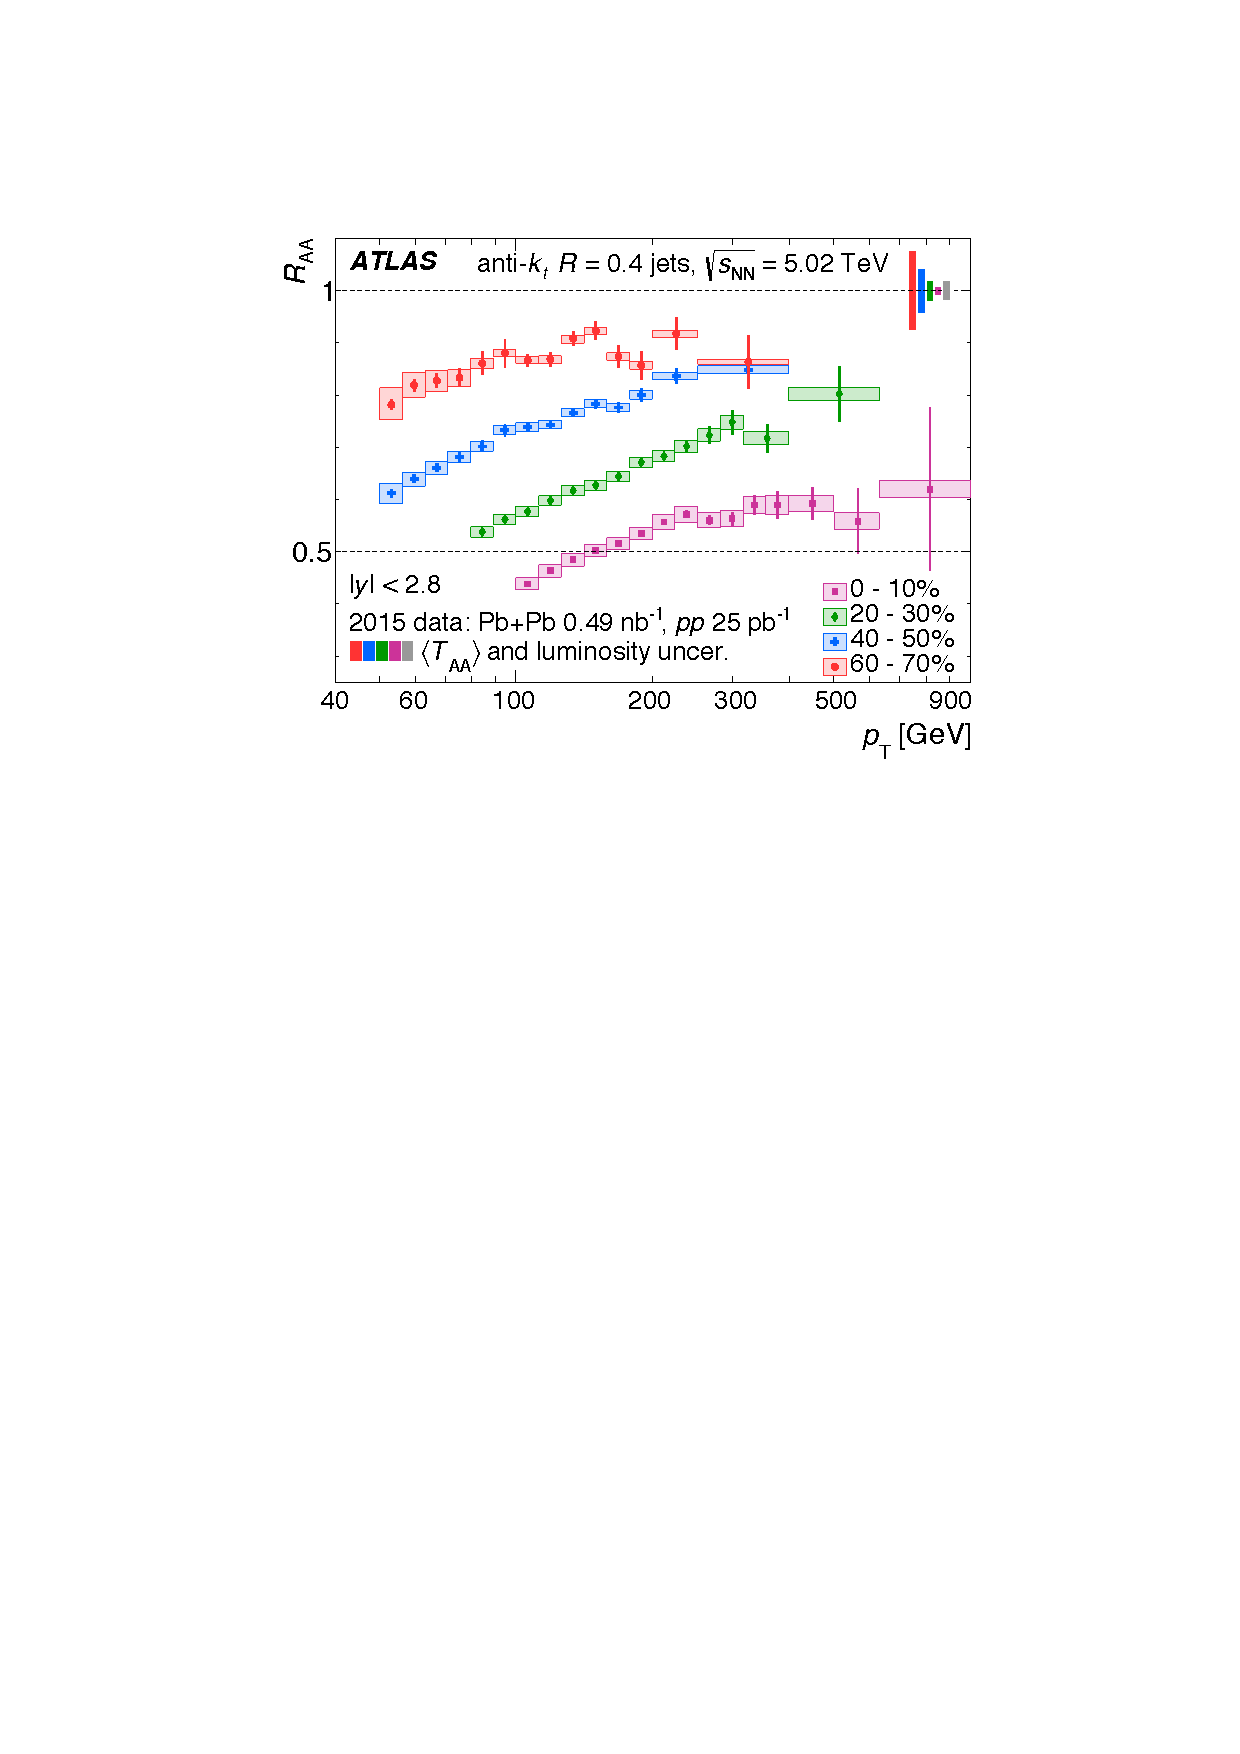
\includegraphics[width=0.55\textwidth]{figures/jetMeasurements/raa}
\caption{The \RAA\ distributions as a function of jet \pt\ for different centrality bins and jet rapidity $|y| < 2.8$. The error bars represent statistical uncertainties while the the shaded boxes represent systematic uncertainties. Figure taken from \cite{2019108}}
\label{fig:raa}
\end{center}
\end{figure}

\begin{figure}[htbp]
\begin{center}
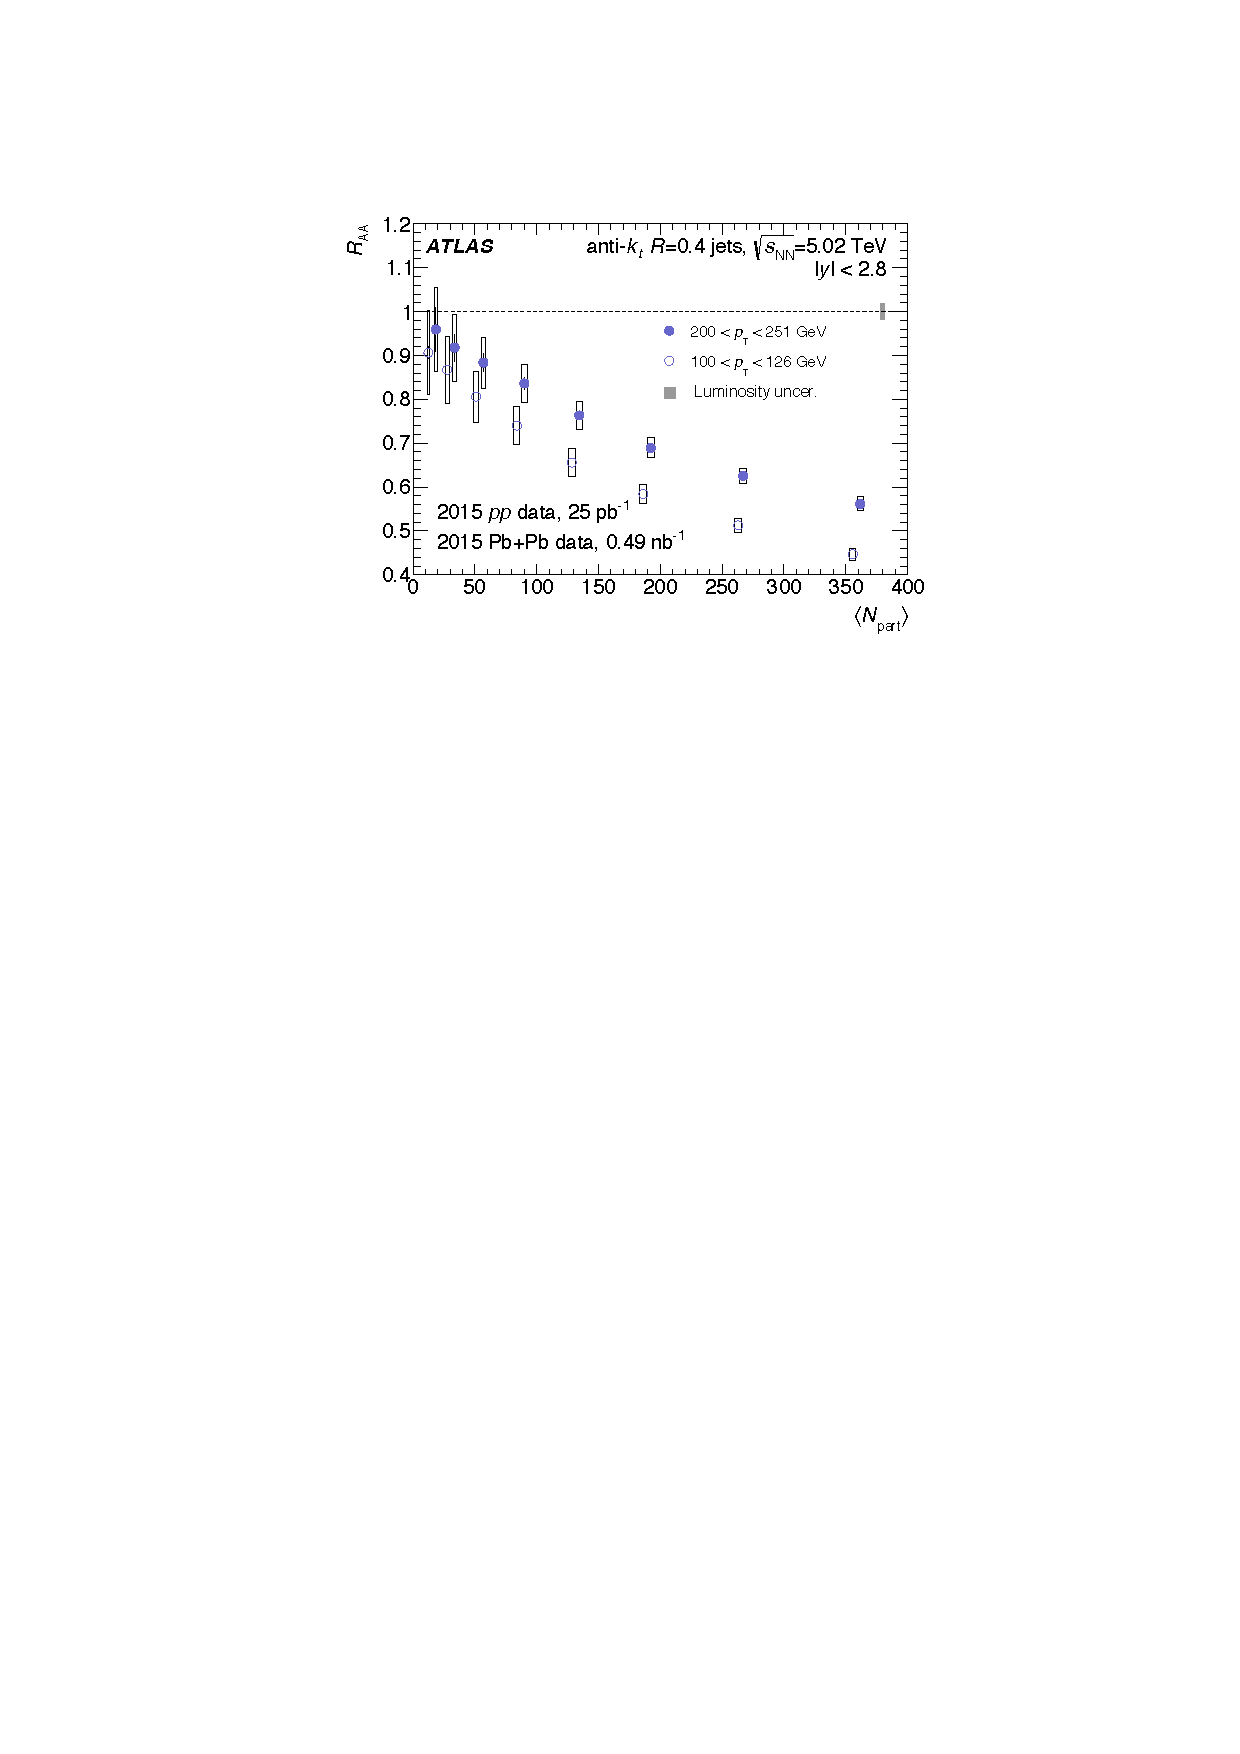
\includegraphics[width=0.55\textwidth]{figures/jetMeasurements/raa_centDep}
\caption{The \RAA\ distributions as a function of jet \pt\ for different centrality bins and jet rapidity $|y| < 2.8$. The error bars represent statistical uncertainties while the the shaded boxes represent systematic uncertainties. Figure taken from \cite{2019108}}
\label{fig:raa_centDep}
\end{center}
\end{figure}









\section{Jet Fragmentation}



